\documentclass[../../main.tex]{subfiles}

% 

\begin{document}
\chapter{Základné charakteristiky spektrometrov}
Spektrometer je vedecké zariadenie pôvodne používané na rozdelenie svetla do jednotlivo oddelených farieb nazývaných spektrum. Spektrometer bol vyvinutý v raných štúdiách fyziky, astronómie a chémie. Spektrometre sa používajú v astronómii na analýzu chemického zloženia hviezd a planét. Koncepcia spektrometra teraz však zahŕňa aj nástroje, ktoré neskúmajú iba svetlo. Spektrometre môžu oddeľovať častice, atómy a molekuly na základe ich hmotnosti, hybnosti alebo energie. Tieto typy spektrometra sa používajú v chemickej analýze a fyzike častíc. Uveďme nejaké základné vlastnosti elektrónových spektrometrov: rozsah merania ($0.01-1000\,keV$), rozlíšenie ($10^{-8}-10^{-1}$), priestorový uhol do ktorého letia detekované elektróny ($0.0001-20 \% $ zo $4\pi$), transmisia T - časť z mono-energetického zväzku elektrónov ktoré prejdú do detektora, intenzita používaných magnetických polí $B=0.0001-3\,T$.

\section{Magnetický spektrometer}
V tomto druhu spektrometra sa magnetické pole využíva na určenie hybnosti (energie) elektrónu, poprípade inej častice. Behom doby boli využívané obzvlášť dva typy magnetických spektrometrov
\begin{itemize}
\item \textbf{Rovinný spektrometer}

Keď rýchlo nabitá častica (náboj $q$, hmotnosť $m$) vstúpi do konštantného magnetického poľa $B$, kde uhol medzi vektorom rýchlosti a vektorom magnetického poľa bude $90^{\circ}$, tak bude v dôsledku Lorentzovej sily vychýlená do kruhovej dráhy o polomere $r$. Moment $p$ tejto častice je potom daný
$$ p=mv=qBr,$$
kde $m$ a $v$ sú hmotnosť a rýchlosť častice, viď obrázok \ref{js6:fig:rovinny_spektrometer}.\par
\begin{figure}[!h]
 \centering
 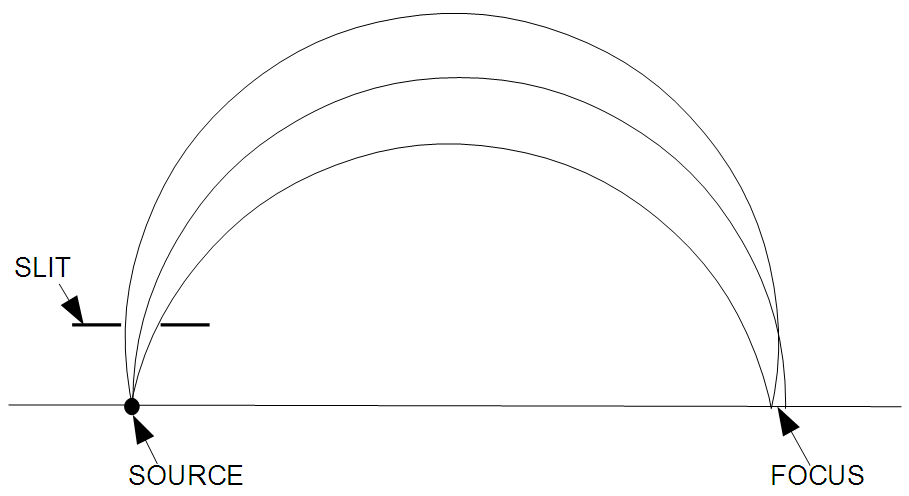
\includegraphics[width=0.5\textwidth]{js6-rovinny-spektrometer.png}
 \caption{Konštantné magnetické pole je kolmé na monitor/list papiera. Nabité častice o hybnosti $p$, ktoré prechádzajú štrbinou sa odchyľujú do  kruhových dráh s polomerom $r=p/qB$. Vidíme, že všetky častice narazili na vodorovnú čiaru na takmer rovnakom mieste. Tu by mal byť umiestnený čítač častíc.}
 \label{js6:fig:rovinny_spektrometer}
\end{figure}
\item \textbf{Šošovkový spektrometer}
V tomto type spektrometra magnetické pole pôsobí ako magnetická šošovka, viď obrázok \ref{js6:fig:sosovkovy_spektrometer}.
\begin{figure}[!h]
 \centering
 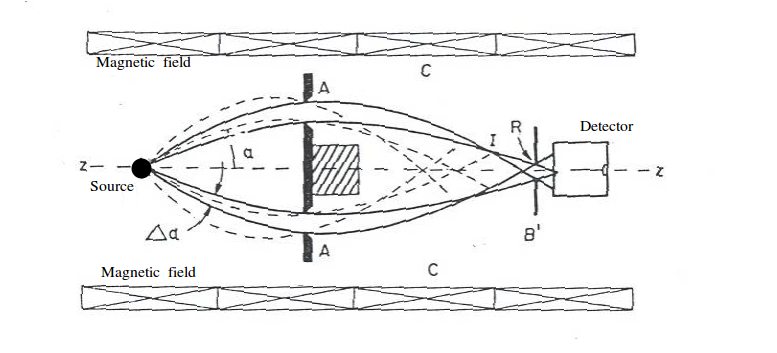
\includegraphics[width=0.9\textwidth]{js6-sosockovy-spektrometer.png}
 \caption{Princíp šošovkového spektrometra.}
 \label{js6:fig:sosovkovy_spektrometer}
\end{figure} \newline
Do tohto typu patri aj tzv. \textit{Orange} alebo \textit{Mini-orange} spektrometer. Tento spektrometer je magnetický, transportný a filtračný systém. Jedná sa o spektrometer, v ktorom magnetické pole usmerní elektróny emitované zdrojom k povrchu detektora, viď obrázok \ref{js6:fig:orange_spektrometer}. Názov tohto zariadenia je spôsobený súborom permanentných magnetov generujúcich pole. Tie sú tvarované ako pomarančové rezy a sú usporiadané v axiálnej symetrii.

Permanentné magnety sú usporiadané symetricky okolo valcového absorbéra (napr. Pb-absorbér). Absorbér chráni detektor proti priamemu žiareniu zo zdroja.
\begin{figure}[!h]
 \centering
 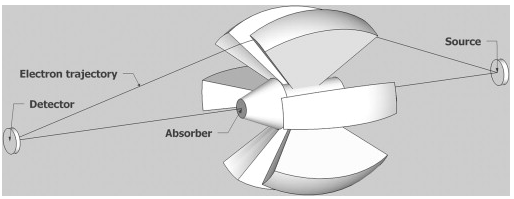
\includegraphics[width=0.7\textwidth]{js6-orange-spectrometer.png}
 \caption{Orange spektrometer: elektróny pochádzajúce zo zdroja sú fokusované na detektor cez toroidné magnetické pole generované súborom permanentných magnetov.}
 \label{js6:fig:orange_spektrometer}
 \end{figure}
Zmenami zostavy magnetov sa dá meniť energia maxima transmisie (tým pádom aj účinnosť spektrometra).

Niektoré spektrometre typu $Orange$ alebo $Mini-orange$ môžu byť využité ako transportéry. Úloha transportéru je nasledovná. Majme prípad kedy meriame na zväzku. V tomto zväzku okrem častíc, ktoré chceme merať, máme aj vysoké pozadie fotónov alebo ďalších častíc. Magnetické pole transportérov je využité na transport elektrónov (alebo iných častíc) mimo toto pozadie. Energia elektrónu je následne určená kremíkovým detektorom. Využíva sa toroidné magnetické pole (pohyb po cykloide) alebo magnetické pole solenoidu (pohyb po špirále). Účinnosť systému je daná transmisiou transportného systému a účinnosťou detektora.
\end{itemize}

\textbf{Rozlíšenie magnetických spektrometrov}\par
Pohyb nabitej častice v magnetickom poli, v ktorom na nabitú časticu pôsobí sila $F_{M}=q\vec{v}\times \vec{B}$. V prípade, keď je vektor $\vec{B}$ kolmý na $\vec{v}$, môžme písať
$$ F=ma=m\frac{v^2}{r}=qvB $$ 
$$ mv=p=qBr $$
$$ R=\frac{\Delta p}{p}=\frac{\Delta(Br)}{Br},$$
kde používame relativistickú hmotnosť elektrónu $m=\frac{m_e}{\sqrt{1-(v/c)^2}}$. Takže $FWHM=\Delta(Br)$ a pre magnetické spektrometre mame rozlíšenie $R=10^{-3}-10^{-2}$.

\section{Elektrostatický spektrometer}
Používa sa pre energie častíc, ktoré nepresahujú $50$ keV. Pre vyššie energie častíc je potrebné príliš veľké napätie a je tu problém aj s relativistickou korekciou. V tomto spektrometre magnetické pole fokusuje elektróny do nejakého konkrétneho miesta, s využitím clon sa robí selekcia hybnosti (energie). Elektrické pole vytvára potenciálovú bariéru, ktorá prepustí elektróny s energiou vyššou ako je istý prah. Avšak, namiesto bariéry sa môže urobiť energetická selekcia častíc tak, že sa budú vyberať elektróny pomocou zakrivenia ich trajektórii v elektrickom potenciály, viď obrázok \ref{js6:fig:elektrostaticky_spektrometer}.
\begin{figure}[!h]
\centering
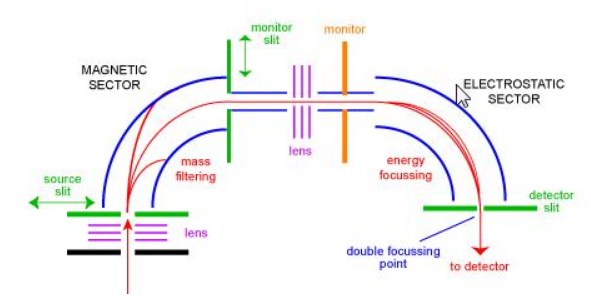
\includegraphics[width=0.9\textwidth]{js6-elektrostaicky-spektroskop.png}
\caption{Magneticky sektor vyberá častice podľa hmotnosti, to sme mali v predchádzajúcom prípade. Avšak, ako vidíme elektrostatický sektor sa zameriava na kinetické energie častíc, kde častice s nevyhovujúcou energiou narazia na steny. Namiesto tej zakrivenej časti môžme mať aj rovnú čast, kde bude nejaká potenciálová bariéra, ktorá nepusti častice, ktorých energia bude pod určitým prahom potenciálu.}
\label{js6:fig:elektrostaticky_spektrometer}
\end{figure}
S týmto elektrostatickým spektrometrom môžme spojiť napríklad tieto detektory:
\begin{itemize}
\item \textbf{Kanálový násobič (channeltron)}\par 
Je vhodný pre nízke energie ($\sim 1\,keV$). Channeltron je vyrobený zo skla alebo keramiky. Povrch je z polovodičovej vrstvy. Zosilenie môže dosahovať hodnoty $\sim 10^7$. Funguje na princípe sekundárnej emisie, kde jeden elektron indukuje emisiu ďalších elektrónov, viď obrázok \ref{js6:fig:channeltron}. Tento násobič má malú citlivosť na detekciu gama žiarenia.
\begin{figure}[!h]
\centering
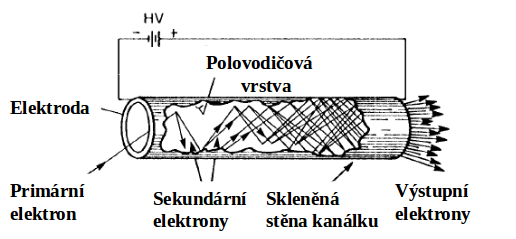
\includegraphics[width=0.9\textwidth]{js6-channeltron.png}
\caption{Primárny elektrón vyemituje niekoľko elektrónov. Tie následne pod vplyvom potenciálu zrýchlia a emitujú ďalšie elektróny. Tento proces beží pokým zosilenie nie je dostatočne.}
\label{js6:fig:channeltron}
\end{figure} \newline
Je tu možnosť zoskupiť viacej channeltronov do tkz. channeltron dosky - milióny miniatúrnych zosilňovačov pracuje nezávisle. Vďaka tejto doštičke vieme určiť polohu častice. Vzdialenosť jednotlivých channeltronov v doštičke je zhruba $\sim 8-30\,\mu m$. Malá citlivosť na magnetické pole a mŕtva doba jednotlivých channeltronov je zhruba $\sim 10$ ns.
\item \textbf{Kremíkové detektory}\par
V tejto časti nebudeme veľmi rozoberať kremíkové detektory pretože sú podrobnejšie popísane v inej otázke. Výhodou týchto detektorov je, že môžu merať ako aj polohu, tak aj energiu daného elektrónu. Poznáme driftové komory, kde náboj z ionizácie driftuje k anóde. Typické driftové rýchlosti sú $\sim 5\,cm/\mu s$, z času letu je možné určiť polohu častice. Ďalej poznáme aj pixlové detektory. Tento detektor sa skladá z jednotlivých pixelov, kde každý pixel má vlastne vyčítanie. Vieme ním určiť veľmi presne polohu. 
\end{itemize}
Príkladom takéhoto elektrostatického spektrometra je ESA12 – elektrostatický spektrometer s vysokým rozlíšením pre elektróny s energiami $0-8$ keV, vhodný pre základné testy elektronových zdrojov vyvíjaných pre projekt KATRIN - experiment zaoberajúci sa neutrínami.\newline
\textbf{Rozlíšenie elektrostatických spektrometrov}\par
Rozlíšenie elektrostatických spektrometrov je rozlíšením energie $R=\frac{\Delta E_{kin}}{E_{kin}}$, kde ${FWHM=\Delta E_{kin}}$. Dá sa ukázať, že vzťah medzi magnetickým a elektrickým rozlíšením je nasledovný 
$$ \frac{dE_{kin}}{E_{kin}}=\bigg( 1+\frac{m_ec^2}{E_{kin}+m_ec^2}\bigg)\frac{d(Br)}{Br},$$ 
kde 
$$ \frac{dp}{p}=\frac{d(Br)}{Br}.$$
V nerelativistickej limite ($E_{kin} << m_ec^2$) máme 
$$ E_{kin}=\frac{p^2}{2m_e} \Rightarrow dE_{kin}=\frac{p}{m_e}dp.$$
Potom dostávame, že 
$$ \frac{dE_{kin}/E_{kin}}{dp/p}=2.$$
Pre ultra-relativistickú limitu ($E_{kin} >> m_ec^2$) dostávame 
$$ E_{kin}=E=pc \Rightarrow \frac{dE_{kin}}{E_{kin}}=\frac{dp}{p}.$$ 
Potom dostávame 
$$ \frac{dE_{kin}/E_{kin}}{dp/p}=1.$$
Graficky vzťah medzi energetickým a hybnostným rozlíšením máme na obrázku \ref{js6:fig:rozslisenie}.
\begin{figure}[!h]
\centering
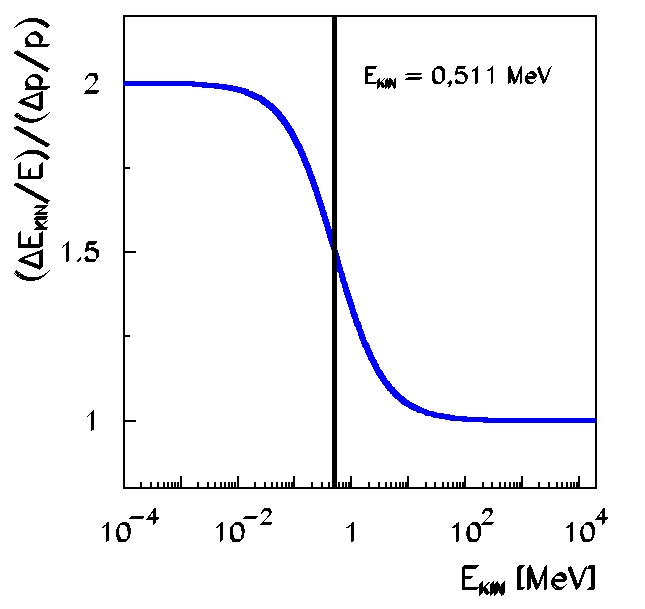
\includegraphics[width=0.5\textwidth]{js6-rozlisenie.png}
\caption{}
\label{js6:fig:rozslisenie}
\end{figure}

\section{Scintilačný spektrometer}
Zariadenie založené na scintilačnom čítači je používané na meranie takých vlastností jadrového žiarenia a elementárnych častíc ako intenzita žiarenia, energia častíc a životnosť nestabilných jadier a častíc. Scintilátory často konvertujú jediný vysoko-energeticky fotón na veľký počet fotónov s nízkou energiou. Meraním intenzity záblesku (počet fotónov vytvorených r\"{o}ntgenovým alebo gamma fotónom) je možne rozoznať pôvodnú energiu fotónu.

Spektrometer pozostáva z vhodného scintilátorového kryštálu, fotonásobovacej trubice a obvodu na meranie výšky impulzov produkovaných fotonásobičom. Impulzy sú spočítané a triedené podľa ich výšky, čím sa vytvorí x-y graf zábleskového scintilačného jasu v porovnaní s počtom zábleskov, ktoré sa približujú energetickému spektru dopadajúceho žiarenia s niektorými ďalšími artefaktmi. Monochromatické gama žiarenie produkuje fotopík pri svojej energii (fotón nestratil ani čast svojej energie). Avšak, nie vždy zachytíme úplne celú energiu žiarenia. Tieto straty sú spôsobené Comptonovským rozptylom. Ďalej v spektre môžme pozorovať dva menšie píky, ktorých energia bude o $0.511\,MeV$ a $1.022\,MeV$ menšia ako pre pôvodný fotón, ktoré zodpovedajú tvorbe elektron-pozitrónového páru, kde jeden alebo oba anihilačné fotóny uniknú z objemu detektora. Ďalej ešte môžme vidieť tkz. beackscatter pík, ktorý vznika, keď fotón interaguje so stenami detektora, pričom prostredníctvom Comptonovského rozptylu alebo fotoefektu vznika žiarenie, ktorého energia je o dosť menšia ako mal pôvodný fotón.

Z dôvodu ich vysokej účinnosti pri zaznamenávaní rôznych častíc a žiarenia a ich rýchlej odozvy sa scintilačné spektrometre široko používajú v jadrovej spektroskopii a spektroskopii častíc s vysokou energiou. Pri nízkych energiách ($\leq1\,MeV$) je energetické rozlíšenie scintilačných spektrometrov nižšie ako pri proporčných počítadlách a polovodičových detektoroch. Kryštály, ktoré sa používajú ako scintilačné materiály, môžu napríklad byť CsI v kryštalickej forme (na detekciu protónov alebo alfa častíc), ZnS (široko sa využíva ako detektor alfa častíc), NaI(Tl) (na detekciu gama žiarenia), LiI (na detekciu neutrónov).

Vo vysoko-energetickej fyzike sa občas používajú veľké segmentové scintilačné spektrometre s úplnou absorpciou na meranie energie prichádzajúcej častice s $~10-100\,GeV$. Hmotnosť scintilátora v takýchto spektrometroch dosahuje desiatky alebo stovky ton. Meranie celkovej energie uvoľnenej v jadrovej kaskáde umožňuje určiť energiu prichádzajúcej častice s presnosťou až do $\pm10\%$.

\section{Polovodičový spektrometer}
Polovodičový spektrometer je zariadenie na meranie rôznych charakteristík jadrového žiarenia a elementárnych častíc. Jeho hlavným prvkom je polovodičový detektor. Polovodičové spektrometre sa používajú napríklad na meranie spektra, žiarenia a na izoláciu jadrových reakcií určitého druhu. Viackanálové analyzátory a elektronické počítače vo všeobecnosti tvoria koncovú časť polovodičového spektrometra. Na dosiahnutie vysokého rozlíšenia energie sa polovodičové spektrometre a predzosilňovače chladia umiestnením do kryostatu. Intenzívne sa využívajú kremíkové ale aj germániové polovodičové detektory. Energetické rozlíšenie týchto detektorov sa pohybuje medzi hodnotami $\sim 0,9-1,9\,keV$ pre častice s energiou $100-1000\,keV$. V závislosti od toho aké hodnoty energie chceme si volíme materiál a hrúbku okienka daného detektora. Na obrázku \ref{js6:fig:BEGe} môžme vidieť prierez germániového detektora, na ktorom vidíme aj spomínané okienko. Materiál a hrúbka okienka sa mení kvôli absorpcii materiálu. V týchto typoch sa využívajú vyššie spomínané magnetické transportéry, ktoré prepravujú elektróny do miesta s menším pozadím. Vo väčších experimentoch ako napríklad LHC, sa využívajú aj pozične citlivé detektory: kremíkové stripové detektory (SSD), kremíkové pixelové detektory (SPD) alebo kremíkové driftové detektory (SDD).
\begin{figure}[!h]
\centering
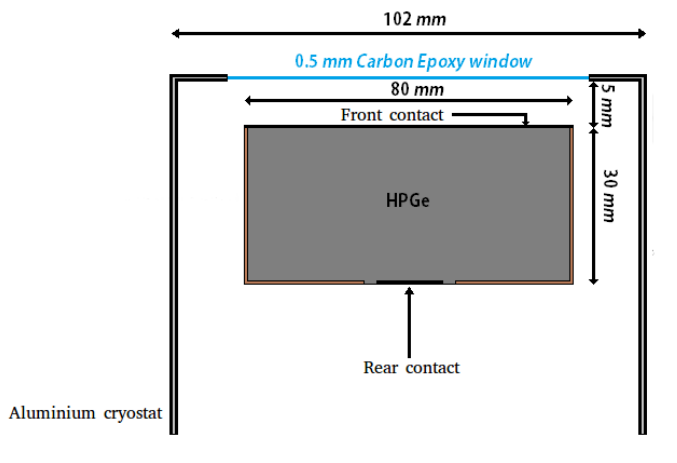
\includegraphics[width=0.4\textwidth]{js6-BEGe.png}
\caption{Prierez germániového detektora typu BEGe. Môžme taktiež vidieť spomínané okienko. V tomto prípade je vyrobene z uhlíka, čo je dobre pre energie menšie ako $10\,keV$. Ďalšie možnosti materiálu pre toto okienko sú napríklad hliník, ktorý je vhodný pre energie väčšie ako $30\,keV$ a pre energie menšie ako $3\,keV$ je najlepšie zvoliť berýliové okienko.}
\label{js6:fig:BEGe}
\end{figure}

Na obrázku \ref{js6:fig:semiconductor_spectrometer} môžme vidieť príklad polovodičového spektrometra, ktorý nesie názov TATRA (TApe TRAnsportation) spektrometer. Bol navrhnutý a skonštruovaný na Fyzikálnom ústave Slovenskej Akadémie Vied. Tento systém pozostáva s vákuovej komory, troch koaxiálnych HPGe detektorov (s $70-80\%$ efektivitou) a jedného Broad Energy Germanium detektora (BEGe), ktoré merali gama žiarenie a jedného Si(Li) detektora, ktorý meral konverzné elektróny s energiou nad $100\,keV$ s rozlíšením $FWHM=1.3\,keV$. Vo vnútri komory je tlak $8\cdot 10^{-8}\,mbar$.

\begin{figure}[!h]
\centering
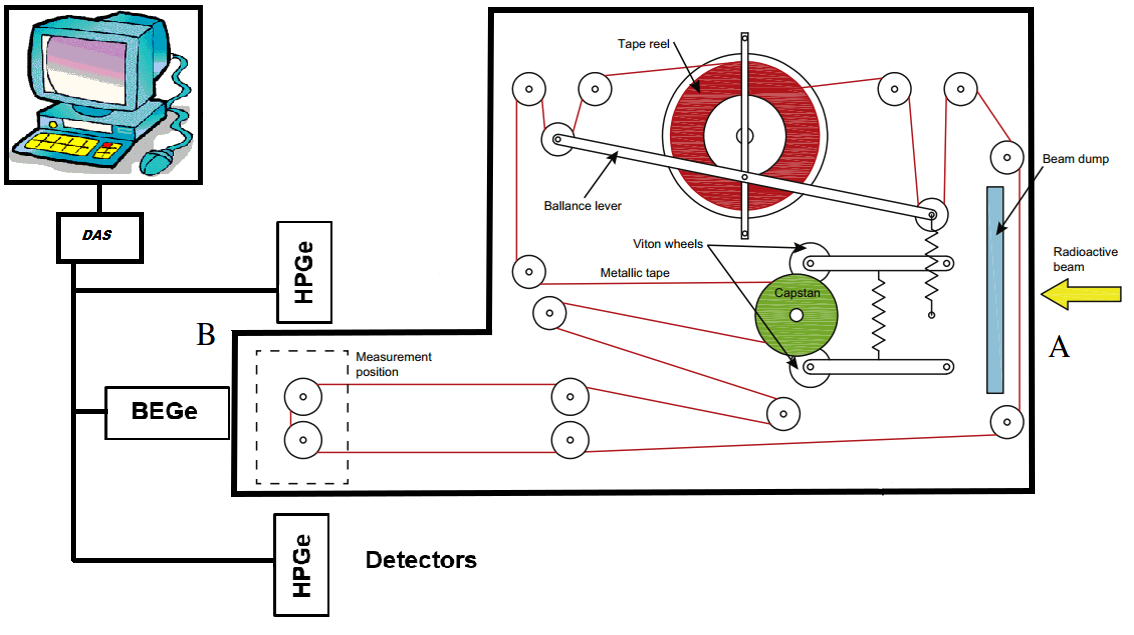
\includegraphics[width=0.8\textwidth]{js6-polovodicove-spektrometer.png}
\caption{Náčrt TATRA spektrometra. Podstatná čast je vo vnútri komory. Následne okolo toho výbežku sú umiestnene detektory, ktoré merajú to, čo je potrebne. Zmerané informácie sú transportované do úložiská. Tento spektroskop nevyužíva magnetické transportéry ale funguje na páskovom princípe, kde sa na jednom mieste naimplementuje vzorka na pásku (bod A) a posunie sa na miesto kde prebieha meranie (bod B).}
\label{js6:fig:semiconductor_spectrometer}
\end{figure}

\section{Kryštálový spektrometer}
Je to röntgenový spektrometer využívajúci kryštálovú mriežku. Tento spektrograf pozostáva z vysokonapäťového napájacieho zdroja ($50\,kV$ alebo $100\,kV$), širokopásmovej röntgenovej trubice zvyčajne s volfrámovou anódou a s berýliovým okienkom a držiakom na vzorku, analyzujúcim kryštálom, goniometrom a detektorom röntgenového žiarenia. Tieto komponenty sú usporiadané tak, ako je to znázornené na obrázku \ref{js6:fig:crystal_spectrometer}. 
\begin{figure}[!h]
\centering
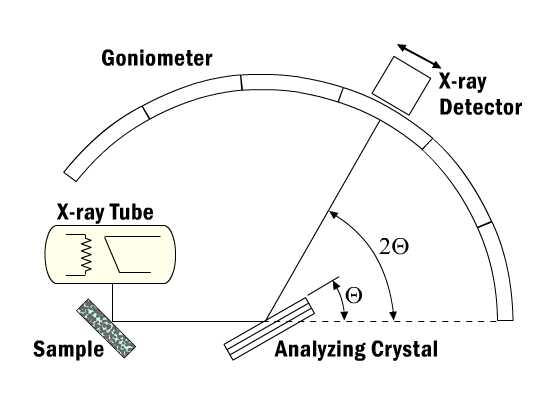
\includegraphics[width=0.5\textwidth]{js6-krystalovy-spektrometer.jpg}
\caption{Schéma kryštálového spektrometra.}
\label{js6:fig:crystal_spectrometer}
\end{figure}
Spojite röntgenové spektrum vychádzajúce z trubice ožaruje vzorku a excituje elektróny vo vzorke, ktoré následne deexcitujú a emitujú charakteristické žiarenie. Každý z 92 prvkov emituje jedinečne charakteristické spektrum. Na rozdiel od optického spektra je röntgenové spektrum pomerne jednoduché. Najsilnejšia čiara, zvyčajne z K-alpha prechodu, ale niekedy aj z L-alpha prechodu, postačuje na identifikáciu prvku. Existencia konkrétnej linky (čiary v spektre) preukazuje existenciu prvku a intenzita je úmerná množstvu konkrétneho prvku vo vzorke. Charakteristické žiarenie sa odráža od kryštálu (analyzátora) pod uhlom, ktorý je daný Braggovým zákonom 
$$ n\lambda = 2d\sin(\theta),$$ 
kde $\theta$ je difrakčný uhol, $n$ je stupeň odrazu ($n=1,2,3...$) a $\lambda$ je vlnová dĺžka žiarenie.
 
Kryštál testuje všetky difrakčné uhly $\theta$ tak, že sa počas merania otáča. Detektor, ktorý zachytáva odrazené žiarenie sa taktiež otáča spoločne s kryštálom. S citlivým detektorom sa röntgenové fotóny počítajú individuálne. Tieto hity sa môžu vykresliť v závislosti od uhla odrazu. Charakteristické röntgenové lúče sa vyskytujú v špecifických uhloch a keďže je známa a zaznamenaná uhlová poloha pre každú röntgenovú spektrálnu čiaru, je ľahké nájsť zloženie vzorky.

\end{document}